%(1) Algorithm
%(2) Time series result and validation
%(3) Deformation maps
%(4) Data now available for stakeholders, what people can do (brief discussion on Peter's work, we could use one of his figures I have).
%



\chapter{Robust Time Series Methods for Long-term Nonlinear Deformation}
\label{CHAP:5-robust-ts}


In this chapter, present a method for robustly extracting slow-moving cumulative surface deformation from time series with large noise. 
We perform a temporal smoothing using the robust Locally Weighted Scatterplot Smoothing (LOWESS) regression technique \cite{Cleveland1979RobustLocallyWeighted} on noisy surface deformation time-series derived using SBAS.
%The method extends the ideas behind the outlier-removal technique presented in Chapter \ref{CHAP:4-GRL}.
Compared to the alternatives presenting in Section \ref{sec:ch4-method-compare}, the LOWESS smoothing more easily accounts for nonlinear deformation while also suppressing the 10-15 cm of tropospheric noise present in the summer SAR acquisitions. 
We demonstrate the technique using synthetic time series and using three paths of Sentinel-1 data over the Permian Basin in West Texas. 
The cumulative results show subtle basin-wide uplift features arising after 4-5 years of heavy sustained wastewater injection.



%- Problem: 
%1. Longer time series, the linear assumption becomes less valid.  This is at odds with the balance of using more measurements to average out tropospheric noise
%2. Methods incorporating temporal smoothness constraints (Find a few. e.g. Karissa? other temp smooth solvers...) or temp lienar filtering methods get influenced by strong tropo days. Even with smoothing, there are anomalous bumps 
%	- can get interpreted as deformation if we assume that all movements remaining after filtering are due to the low-pass deformation
%	

\section{Algorithm}
%	\bm{A \phi} = \bm{\Delta \phi} + \bm{\epsilon} . \label{eq:ch2-sbas-A}
%where  $\bm{A}$ is the system design matrix, and $ \bm{\epsilon}  $ is the vector of interferogram-specific noise sources (e.g. $ \Delta \phi_{decor}, \Delta \phi_{unwrap}, \Delta \phi_{scat}, \Delta \phi_{n} $ from Equation \eqref{eq:ch2-insar-noise-terms}).
Consider a time series of $N$ LOS phase delays for a single pixel,  $ \bm{\phi} = \left[\phi_0, \phi_1, \ldots, \phi_{N-1} \right]^T $ sampled at time intervals $ \bm{t} = \left[t_0, \ldots, t_{N-1} \right]^T $, solved from the SBAS linear system (Equation \eqref{eq:ch2-sbas-A}).
We can write each element $\phi_i$ as a sum of surface deformation and atmospheric delay,
\begin{equation}
	\phi_i = \frac{4 \pi}{\lambda} \left(d_i + \alpha_i \right)
\end{equation}
where $ d_i$ and $\alpha_i$ are the surface deformation and atmospheric delay on the $i$th day, and $ \lambda $ is the radar wavelength.
Here we consider the case that the interferogram-specific noise sources (e.g. $  \Delta \phi_{decor}, \Delta \phi_{unwrap}, \Delta \phi_{scat}  $) have been properly accounted for in the inversion process so that the remaining noise in  $ \bm{\phi} $ is predominantly from the atmospheric delay $ \bm{\alpha} =\left[\alpha_0, \ldots, \alpha_{N-1} \right]^T $.
%Since deformation is usually the quantity of interest,
Our goal is to separate the vector of surface deformation $ \bm{d} =  \left[d_0, d_1, \ldots, d_{N-1} \right]^T $ from the atmospheric noise $ \bm{\alpha} $.
% consists of all terms in Equation \eqref{eq:ch2-insar-noise-terms} which affect the phase of a SAR acquisition and all interferograms containing that acquisition

The most widely used non-parametric methods for separating $ \bm{d} $ from $ \bm{\alpha} $ rely on the fact that the turbulent component of $\bm{\alpha}$ is uncorrelated in time, while most deformation sources show strong temporal correlation.
%There are several approaches to separating $ \bm{d} $ from $ \bm{\alpha} $.
%If a functional model of deformation is known to exist (e.g. linear, transient jumps \citep{Chen20142010SlowSlip, Fielding2017SurfaceDeformationNorth}, seasonal variations \citep{Murray2018ShortLivedPause}, or a combination \citep{Riel2018QuantifyingGroundDeformation}), a model fit can be performed on the noisy $ \bm{\phi} $ time series to extract the model parameters of interest.
%However, when the deformation model is not known, methods usually rely on the fact that the turbulent component of $\bm{\alpha}$ is uncorrelated in time \citep{Emardson2003NeutralAtmosphericDelay} while most deformation sources show strong temporal correlation.
For example, the authors of \cite{Ferretti2000NonlinearSubsidenceRate} and \cite{Berardino2002NewAlgorithmSurface} estimated $\bm{\alpha}$ by performing a high-pass temporal filter on each pixel followed by spatially low pass filtering the residual phase.
The temporal high pass filter was implemented by subtracting a low-pass filtered version of $ \bm{\phi} $ (using a triangular filter in \cite{Ferretti2000NonlinearSubsidenceRate}) from the original unfiltered version.
% (i.e. $ \phi $)
%used spatial and temporal filters on $\bm{\Delta \phi}$.
%These filters are expanded upon and compared in Chapter \ref{CHAP:5-robust-ts}, where a new robust filter is presented to separate deformation from atmospheric noise.
One difficulty with the triangular filter and other moving-average filters (e.g. a Gaussian filter) is that the filter coefficients are non-adaptive; noisier atmospheric conditions will be weighted the same as calmer conditions \citep{Liu2012SatelliteRadarInterferometry}.
This can cause considerable leakage of noise from severe weather conditions (e.g. thunderstorms) into the deformation estimate of adjacent days.

% From Liu, 2012
% Given a good spatial density of coherent targets and a short satellite repeat orbit the filtering method used in the standard PSInSAR (see Ferretti et al. (2000)) provides a simple and fast means to separate APS from temporally correlated deformation signal. However, the separation is usually not optimal and can be erroneous when there are acquisition gaps in the time series or for acquisitions taken under extreme weather conditions such as thunderstorms. This is because the approach weights APS equally for all acquisitions and remove it by a window-based (e.g., triangle, Gaussian) temporal low-pass filter. The filter is not adaptive and its parameters (e.g., temporal correlation length) are up to the users to specify. A good filter, however, should weight APS per acquisition differently according to its significance and be self-adjustable based on the input data to optimize its parameters towards an optimal filtering.


\begin{figure}
	\centering
	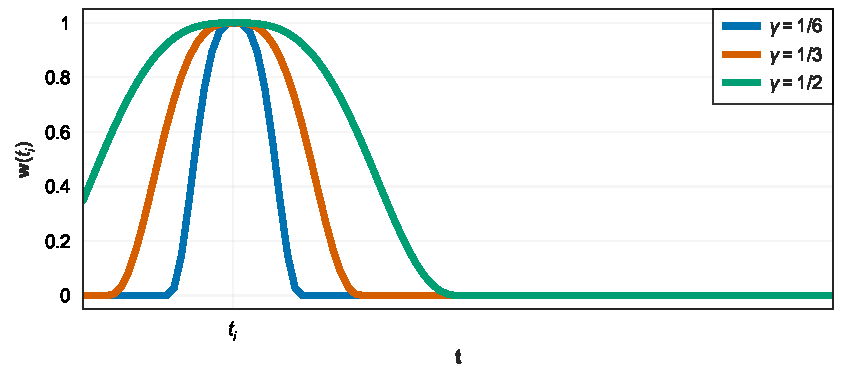
\includegraphics[width=.99\textwidth]{figures/chapter5-lowess/figure1-window.pdf}
	\caption[LOWESS tricube weighting function]{
		LOWESS tricube weighting function $ \bm{w}(t_i) $ for an inclusion fraction of $ \gamma = 1/6 $ (blue), $ \gamma = 1/3 $ (orange), and $ \gamma = 1/2 $ (green).
	}
	\label{fig:ch5-algo-window}
\end{figure}


We can adaptively filter the noisy $ \bm{\phi} $ time series by implementing a robust LOWESS regression \citep{Cleveland1979RobustLocallyWeighted}. The LOWESS algorithm fits a local linear regression at every $t_i$ using nearby data points, repeating over multiple iterations to refine the fit and reduce the effect of outliers \citep{Efron2019ComputerAgeStatistical}.
% which performs several iterations of weighted linear regression for each SAR acquisition. 
For the first iteration, at each time $t_i$,  we calculate a set of weights $\bm{w}(t_i)$. The weight function has a maximum value of $1$ at $t_i$ and decays to zero at the $r$th nearest neighbor to $t_i$, where $r = \left\lfloor \gamma N \right\rfloor$, $0 < \gamma \leq 1$ is the fraction of the data chosen to include for each local fit, and $ \left\lfloor x \right\rfloor $ is rounds $ x $ down to the next lowest integer.
Let $h_i$ be the $r$th smallest number of $\left| x_i - x_k \right|$ for $ k = 0, \ldots, N-1 $.
The $k$th weight $w_k(t_i)$ is defined as
\begin{equation}
	w_k(t_i) = 
	\begin{cases}
		\left( 1 - \left|\frac{t_i - t_k}{h_i} \right|^3 \right)^3 , & \text{if}\  \left|\frac{t_i - t_k}{h_i} \right| < 1 \\
		0, & \text{otherwise}
	\end{cases}          \label{eq:ch5-lowess-weights}
\end{equation}
for $k =0, \ldots, N-1 $. This weight function is known as the \emph{tricube} weighting function.
Figure \ref{fig:ch5-algo-window} illustrates the shape of  $ \bm{w}(t_i) $ for $\gamma = 1/6, 1/3$ and  $1/2 $.



Using $ \bm{w}(t_i) $, we compute a weighted linear regression around $t_i$ by finding the intercept and slope, $a_i, b_i$ that minimize
%\begin{equation}
%		\begin{bmatrix}
%		1, t_0 \\
%		1, t_1 \\
%		\ldots \\
%		1, t_{N-1} \\
%	\end{bmatrix}
%	\begin{bmatrix}
%		a_i \\ b_i
%	\end{bmatrix}
%= \bm{\phi}
%\end{equation}
\begin{equation}
	\sum_{k=0}^{N-1} w_k(t_i) \left(\phi_k - a_i - b_i t_k \right)^2
\end{equation}
The smoothed estimate $\hat{\phi}_i$ at the point $t_i$ is calculated as $\hat{\phi}_i = a_i + t_i b_i$. This process is repeated for all $t_i$,  $i = 0, \ldots, N-1$.

The second iteration performs another weighted least squares fit, this time further downweighting based on the residuals of the first iteration.
Let $\epsilon_k = \left| \hat{\phi}_k - \phi_k  \right|$ be the residual at $t_k$ and $s$ be the median residual for all $k$. We create an additional set of weights $ \delta_k $ for each $ k = 0, \ldots, N-1$ as
\begin{equation}
	\delta_k = 
	\begin{cases}
		\left( 1 - \left(\frac{ \hat{\phi}_k - \phi_k }{6 s} \right)^2 \right)^2 , & \text{if}\  \left( \frac{ \hat{\phi}_k - \phi_k }{6s} \right) < 1 \\
		0, & \text{otherwise}
	\end{cases}          \label{eq:ch5-lowess-weights2}
\end{equation}
Equation \eqref{eq:ch5-lowess-weights2} uses the median $ s $ so that large outliers are clipped to 0, similar to the use of the median absolute deviation from Section \ref{sec:ch4-outlier-method}. For each new fit in the second iteration, the weights $ \bm{w}(t_i) $ are multiplied by the residual weights $\bm{\delta}$ to perform the local regressions.

Finally, we perform a shift of $ \bm{\hat{\phi}} $ to compensate for the first day's atmospheric conditions by taking $ \hat{\phi}_i = \hat{\phi}_i - \hat{\phi}_0 $ for all $ i = 1, \ldots, N-1 $.
This step is necessary for $ \bm{\phi} $ solved using the SBAS formulation of Equation \eqref{eq:ch2-sbas-A}, which assumes the first date's phase is equal to 0, causing $ \alpha_0 $ to be present in all dates.
While \cite{Ferretti2000NonlinearSubsidenceRate} uses mean value of the common-reference interferogram phases as an estimation of the first date's atmospheric noise, here we use the y-intercept of the smoothed time series, $ \hat{\phi}_0 $, as an estimate of $ \alpha_0 $. 


%
%%$ \bm{v} = (\bm{A}^T \bm{A})^{-1}\bm{A}^T \bm{\Delta \phi} $
%%As noted in \cite{Simons2007InterferometricSyntheticAperture}, 
%The least squares solution $ \bm{v} = (\bm{B}^T \bm{B})^{-1}\bm{B}^T \bm{\Delta \phi} $ (or minimum norm solution n $ \bm{v} = \bm{B}^{\dagger} \bm{\Delta \phi}$ ) from \cite{Berardino2002NewAlgorithmSurface} assume that all measurements in $\bm{\Delta \phi}$ have equal variance; subsequent authors have implemented a weighted least squares solution:
%\begin{equation}
%	%	\bm{\phi} = \bm{A}^{\dagger} \bm{\Delta \phi}
%	%	\bm{\phi} = (\bm{A}^T \bm{\Sigma}^{-1} \bm{A})^{-1}\bm{A}^T \bm{\Sigma}^{-1} \bm{\Delta \phi}  \label{eq:ch2-sbas-wls}
%	\bm{v} = (\bm{B}^T \bm{\Sigma}^{-1} \bm{B})^{-1}\bm{B}^T \bm{\Sigma}^{-1} \bm{\Delta \phi}  \label{eq:ch2-sbas-wls}
%\end{equation}
%where $ \bm{\Sigma} = \mathbb{E}[\bm{\epsilon} \bm{\epsilon}^T] $ is the measurement covariance matrix.



%
%\begin{figure}
%	\centering
%%	\includegraphics[width=.99\textwidth]{figures/chapter5-lowess/figure1-demo.pdf}
%	\caption[Multiple iterations of LOWESS fit]{
%		(a) First round fit at one $ x $ location (Same as Figure \ref{fig:ch5-algo-demo}c)
%		(b) Additional weights imposed from the residuals of first fit
%		(c) New weighting window
%		(d) Improved fit from second and third iterations
%	}
%	\label{fig:ch5-algo-iteration}
%\end{figure}


% TODO: The first date of SBAS?


\begin{figure}[!h]
	\centering
	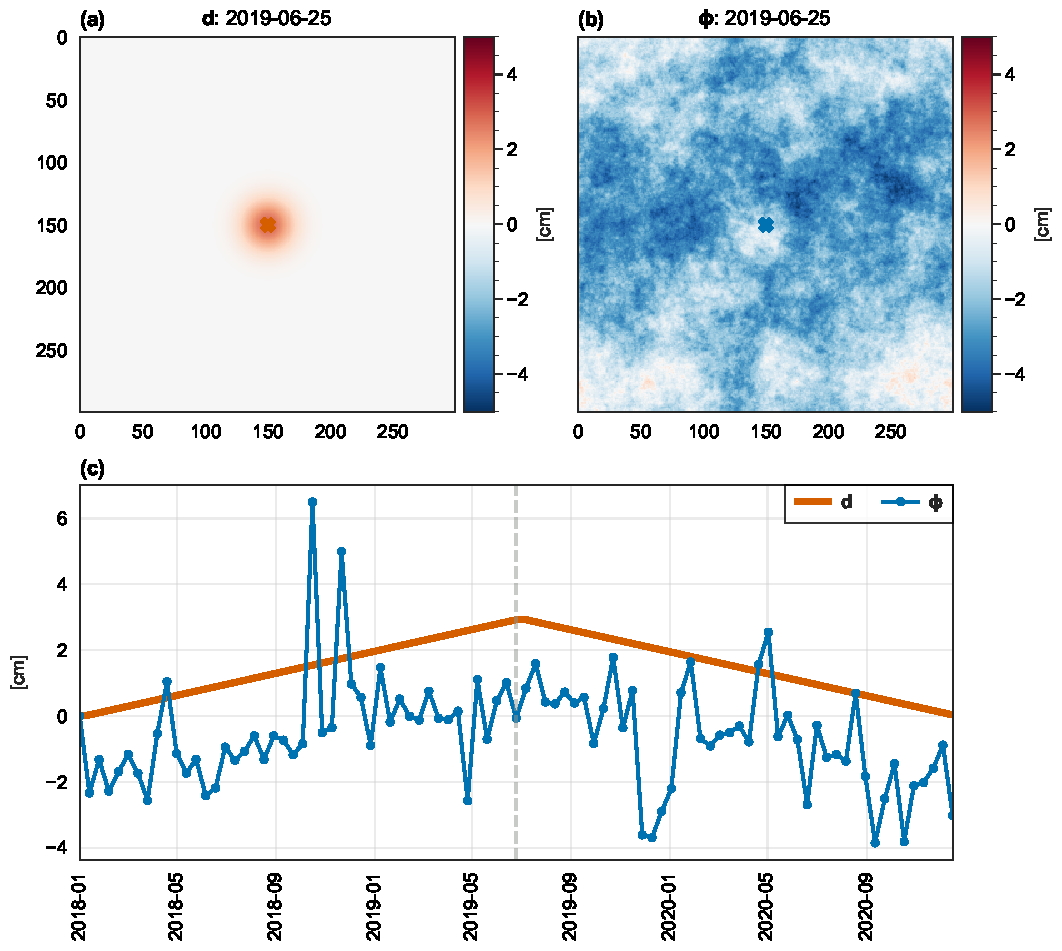
\includegraphics[width=.99\textwidth]{figures/chapter5-lowess/figure2-demo-data.pdf}
	\caption[Synthetic data for LOWESS smoothing]{
		(a)  A 300 x 300 pixel region contains a synthetic uplift bowl which peaks at 3 cm.
		(b) Turbulent tropospheric is noise added to panel (a) for 
		(c) Time series of true deformation $\bm{d}$ (orange) and $\bm{\phi} =\bm{d} + \bm{\alpha}$ (green). The pixels where the $\bm{d}$ and $\bm{\phi}$ time series are drawn from are marked with an x in panels (a) and (b), respectively. The date that panels (a) and (b) are plotting from is marked with the grey dashed vertical line. Note that the $ \bm{\phi} $ time series is offset due to SBAS assuming the first date is $ 0 $.	
	}
	\label{fig:ch5-demo-data}
\end{figure}

\section{Synthetic Example}


We first illustrate the LOWESS algorithm on a synthetic 3-year deformation time series (Figure \ref{fig:ch5-demo-data}).
A 300 x 300 pixel region contains an uplift bowl which linearly increases to $ 3 $cm max after 1.5 years (Figure \ref{fig:ch5-demo-data}a) and deflates back to zero by the end of 3 years. Turbulent tropospheric noise is simulated for acquisitions every 12 days and added to the deformation (Figure \ref{fig:ch5-demo-data}b). The uplift bowl inflates at a constant rate for 1.5 years, then deflates back to 0 by the end of the 3rd year (Figure \ref{fig:ch5-demo-data}c).
To emulate the output from an SBAS inversion, the sum of the deformation and noise is shifted by the noise on the first day so that $ \phi_0 = 0 $.




Figure \ref{fig:ch5-algo-demo} illustrates two iterations of the LOWESS algorithm the $ \bm{\phi} $ time series from(Figure \ref{fig:ch5-demo-data}c).
During the first iteration, each $ \hat{\phi}_i $ is calculated using a locally weighted regression, with the weight based solely on the proximity to $ t_i $ (Figure \ref{fig:ch5-algo-demo}a). The resulting fit tracks the slowly varying pattern of the data, but outlier points can strongly influence the fit (Figure \ref{fig:ch5-algo-demo}b). 
%Using the residuals of the fit from Figure \ref{fig:ch5-algo-demo}b, 
The second iteration combiners the proximity weighting from Figure \ref{fig:ch5-algo-demo}a with the residual weighting calculated from Figure \ref{fig:ch5-algo-demo}b, $ \bm{\delta} $ (Figure \ref{fig:ch5-algo-demo}c).
The second iteration gets influenced less by the outlier points and has fewer spurious bumps in the time series (Figure \ref{fig:ch5-algo-demo}d). Note that more iterations can be performed if desired; in this example, further iterations provide little benefit ($ \sim $ 1 mm or less).


\begin{figure}
	\centering
	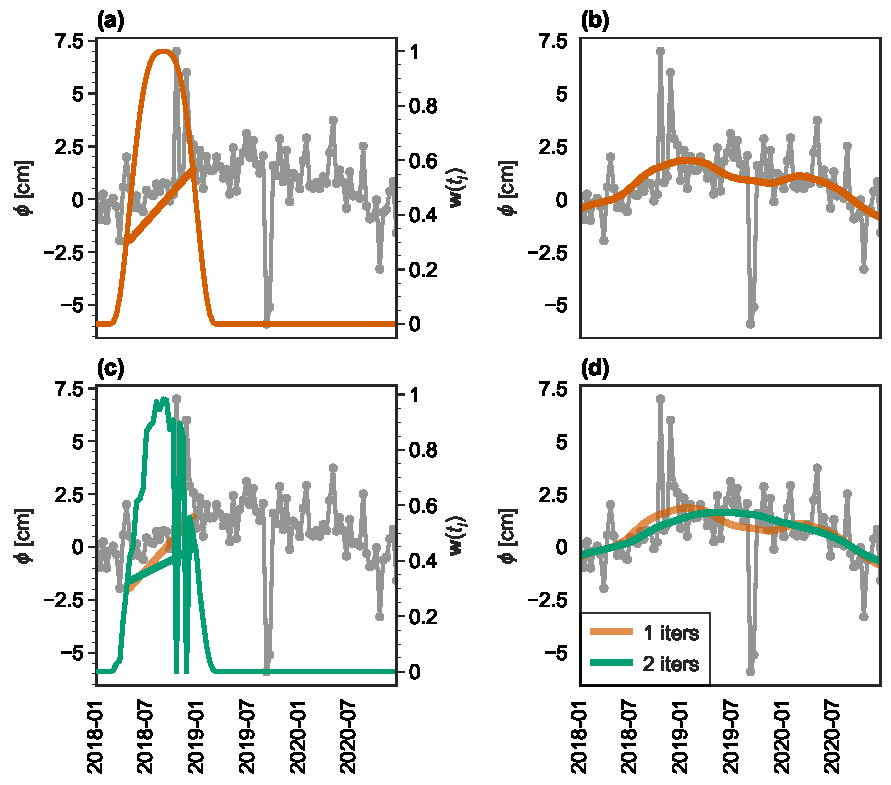
\includegraphics[width=.99\textwidth]{figures/chapter5-lowess/figure3-fits.pdf}
	\caption[Demo of LOWESS fitting]{
		(a) First iteration of local fit at $t_i$, weighted by window (orange) with $ \gamma=0.4 $ ($ \sim $1.2 year of data). Shading of dots indicates the weight factor, where gray indicates 0 weighting and gold indicates full weighting.
		(b) First iteration of smoothed $ \hat{\phi}_i $ (orange line) for all $i$. 
		(c) Second iteration at $t_i$, where the weighting combines the original window with the updated residual weighting. The large anomalous points have a smaller effect on the new local fit (green slope) compared to the original (orange slope).
		% to produce a new weighted least squares fit.
		(d) Result of second iteration of LOWESS smoothing for all $i$ (green line).
	}
	\label{fig:ch5-algo-demo}
\end{figure}

\FloatBarrier


\begin{figure}[!h]
	\centering
	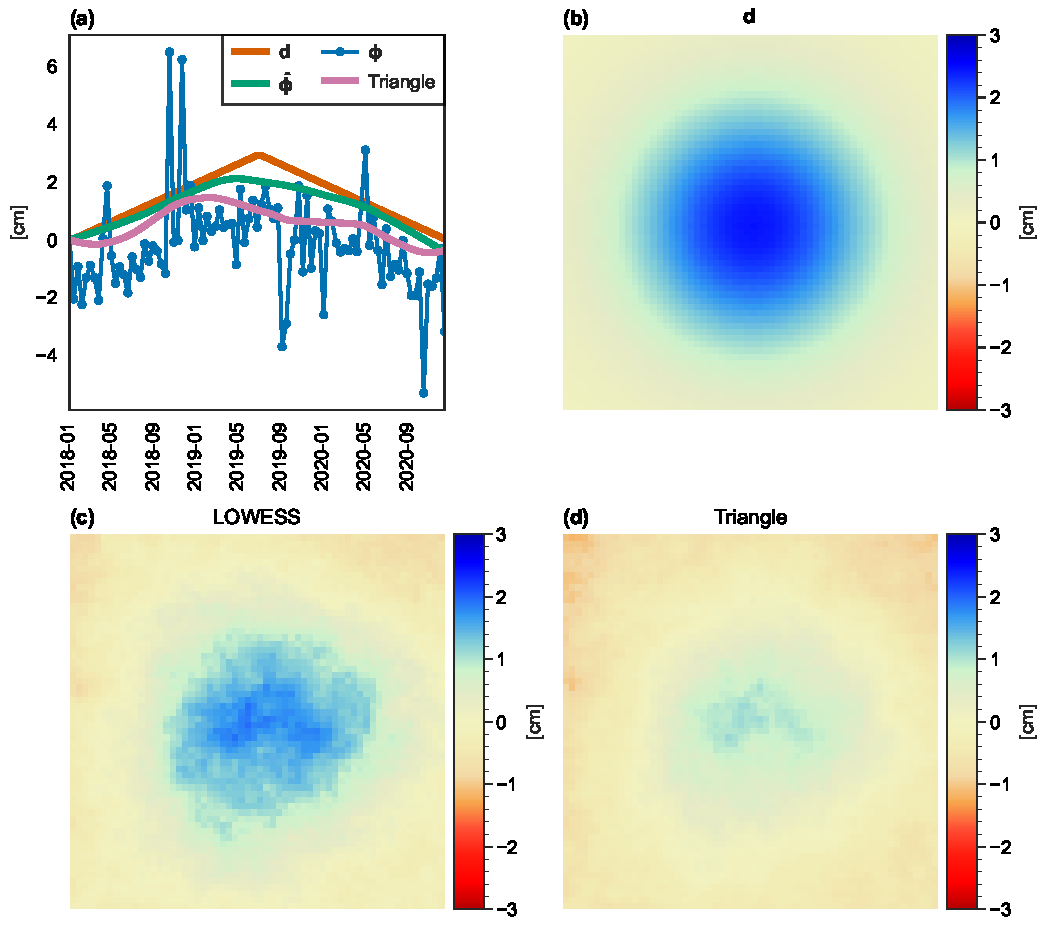
\includegraphics[width=.99\textwidth]{figures/chapter5-lowess/figure4-compare-tri.pdf}
	\caption[Comparison of LOWESS smoothing to triangle filter for synthetic data]{
Results of smoothing the synthetic noisy time series $ \bm{\phi} $ (blue with dots) using the LOWESS algorithm (green) and a triangle filter (pink). True deformation time series is shown in orange.
 Both the LOWESS algorithm and the triangle filter use $ 40 $\% of the data (a filter width of $ \sim $1.2 years) and have been shifted to compensate the first day's atmospheric noise.

	}
	\label{fig:ch5-compare-tri}
\end{figure}

After subtracting $ \phi_0 $ from all points, the results of the LOWESS estimate $ \bm{\hat{\phi}} $ are shown in Figure \ref{fig:ch5-compare-tri}a (green line). The LOWESS algorithm smooths away the large spikes of turbulence noise in  $ \bm{\phi} $ Figure \ref{fig:ch5-compare-tri}a (blue). We note that since the width of the weighting window $ \bm{w} $ was slightly over 1 year, the algorithm smooths over the peak of the deformation lasting several months (Figure \ref{fig:ch5-compare-tri}a, orange line), but captures most of the deformation signal (Figure \ref{fig:ch5-compare-tri}c).
For comparison, we have also smoothed the noisy time series with a 1.2 year wide triangle filter (Figure \ref{fig:ch5-compare-tri}a pink line). The triangle filter performs similarly to LOWESS when the noise is Gaussian; however, in this example with several large turbulence jumps, the triangle filter is pulled $>2$ cm away from the true deformation time series (Figure \ref{fig:ch5-compare-tri}d).


\section{InSAR Processing for Sentinel-1}

%TODO: do I show the 3-path example?

%%For Sentinel-1 path 78, we processed all interferograms with temporal baselines less than 500. 
%%Since all interferograms had less than 250 meter spatial baseline, we required no maximum spatial baseline threshold.  
%%We unwrapped each interferogram using the Statistical-cost, Network-flow Algorithm for Phase Unwrapping (SNAPHU).
%
%We use the Path 78 and Path 85 inteferograms from Section .
%We reduce long wavelength and stratified tropospheric noise by removing a combined planar phase ramp and linear phase vs. elevation relation \cite{Doin2009CorrectionsStratifiedTropospheric, Zebker2021AccuracyModelFree}. We used the mean of the pixel values in a window around GPS station TXKM as a reference.
%We repeated this process for descending path 85 and ascending path 151. Since path 151 does not contain station TXKM, or any other GPS station near the center of the acquisition, we used the referencing technique presented in \cite{Zebker2021AccuracyModelFree} to fit and remove a phase-elevation trend from all high-coherence pixels in each interferogram. This method relies on the assumption that most pixels in each interferogram do not show significant deformation, which is valid Path 151 which only partially overlaps with the western portion of the oil-producing Permian Basin. 
%%our signals deform slowly over time

%FIGURE: 3 path study

%For each pixel, we solved for the cumulative line of sight path delay for all SAR acquisition dates using the SBAS linear system.
%The path delay consist of the true relative surface deformation on each date and a tropospheric noise component, which can lead to jumps of 10 cm or more between consecutive dates.
%Since the atmospheric noise is correlated in space but uncorrelated in time, previous authors have isolated and mitigated the atmospheric noise by using a high pass temporal filter followed by a 2D spatial low pass filter
%\cite{Ferretti2000NonlinearSubsidenceRate, Ferretti2001PermanentScatterersSar, Berardino2002NewAlgorithmSurface, Hooper2012RecentAdvancesSar}.
%Here we perform a temporal smoothing using the robust locally weighted regression (LOWESS) method \cite{Cleveland1979RobustLocallyWeighted}. For each pixel, LOWESS performs multiple iterations of weighted linear regression at each point in the time series. The method weights nearby points more heavily than far away points. We use a window size such that at least two years of SAR acquisitions are weighted for each date, with more points considered during times of regular acquisitions.
%Subsequent iterations use the residuals of the data points from the smoothed line to further deweight noisy acquisitions. Points with residuals larger than 6 times the median absolute residual are clipped to have 0 weight in future iterations. In this manner, the smoothing is robust to strong tropospheric turbulence noise that would otherwise leak into neighboring days using a moving average temporal filter. Additionally, since LOWESS assumes no underlying model, the smoothing can accommodate nonlinear deformation.
%
%To mitigate final residual long wavelength tropospheric noise, we remove quadratic ramp from the phase of each date in the time series (where we mask out pixels with $>$2 cm of estimated deformation to avoid removing deformation) \cite{Morishita2020LicsbasOpenSource}.

\section{Results}

\subsection{Permian Basin 7-year time series}

\subsection{GPS comparison}

\section{Discussion}

%1. Limitations of stacking to long time series
%2. Robust Time Series Methods
   %1. Regularization (Supplement from GRL)
   %2. LOWESS smoothing
%3. Synthetic Example
%4. 7 Year Time Series for the Permian Basin
%1. Comparison to GPS
%2. Anthropogenic Caused Deformation Patterns


%Problems with pixelwise uq
%- Image of blob, with 8 mm cutoff, question which part you trust and not
%- Leads into feature-wise uq




